\documentclass[12pt,a4paper]{article}
\usepackage[a4paper,top=12mm,bottom=16mm,left=15mm,right=15mm,footskip=8mm]{geometry}
\usepackage[T1]{fontenc}
\usepackage{amsmath}
\usepackage{amssymb}
\usepackage{cancel}
\usepackage{enumitem}
\usepackage{multicol}
\usepackage{array}
\usepackage{xcolor}
\usepackage{tikz}
\usepackage[most]{tcolorbox}
\usetikzlibrary{arrows.meta,decorations.pathreplacing}

% ================================================================
% Worked solutions to "An Introduction to Indices and Roots".
%
% Every question and every lettered part of the worksheet is worked
% through here, in the order in which it appears on the sheet, and the
% method used is the method taught in the worked example that comes
% before the question, laid out in the same steps, so that a pupil can
% line their own working up with the solution line by line.
%
% Cancelling is shown the way the worksheet shows it: the numerator
% and the denominator are written as multiplications and each factor
% that appears in both is crossed out with \cancel. When every factor
% on the bottom cancels, the denominator is written as 1 rather than
% left blank, and the fraction is then written as its numerator. The
% factorial questions are done by writing both factorials out in full
% and cancelling, not by working the factorials out first.
%
% The two match-ups, Q1 and Q7, are given as the calculation for each
% numbered item together with the letter it joins to. The open ended
% parts, Q2(f), Q6(i), Q8, Q9(b), Q12, Q13(b) and (c), Q14(d), and
% Q15(g) and (i), are
% given a model answer in full sentences followed by a note of what
% else would be accepted.
%
% Six "Common mistake" boxes sit beside the solutions where the most
% likely errors show. Each one names the mistake and draws a picture
% that settles it: arrays of squares for reading an index as a
% multiplier, return arrows for dividing by the index to find a root,
% factor tiles for counting the number in front as part of the index,
% pairing arrows for cancelling by column, crossed-out factors with a 1
% left behind for "cancelled means nothing", and paired minus signs for
% the sign of a power of a negative number. They were found by working
% the sheet through as a weaker pupil would, and are kept here rather
% than on the worksheet so that the worksheet stays uncluttered.
%
% The headings and the boxes are the ones used on the worksheet, and
% are tinted only faintly, with pale title bars and coloured title
% text, so that the solutions are cheap to print. The \newpage
% commands are placed so that no solution is split across a page
% break.
% ================================================================

\linespread{1.12}\selectfont
\setlength{\parskip}{4pt}
\setlength{\parindent}{0pt}
\setlist[enumerate,1]{label=(\alph*), leftmargin=*, itemsep=6pt,
  topsep=4pt, parsep=3pt}
\setlength{\multicolsep}{4pt}

% A worked example: the method shown in full before it is practised.
% The boxes are tinted only faintly, and their title bars are pale with
% coloured text rather than solid, so that the sheet is cheap to print.
\newtcolorbox{wex}[1]{colback=blue!1,colframe=blue!45!black,boxrule=0.6pt,
  colbacktitle=blue!8,coltitle=blue!50!black,
  left=6pt,right=6pt,top=4pt,bottom=5pt,
  title={\bfseries\small Worked example: #1},fonttitle=\small,
  toptitle=1pt,bottomtitle=1pt}

% The idea a section is built on, stated once and boxed.
\newtcolorbox{keyidea}{colback=orange!2,colframe=orange!60!black,boxrule=0.6pt,
  left=6pt,right=6pt,top=4pt,bottom=4pt}

% The notation for a section, set out so that it can be found again
% from anywhere on the sheet.
\newtcolorbox{notation}[1]{colback=green!1,colframe=green!35!black,boxrule=0.9pt,
  colbacktitle=green!10,coltitle=green!30!black,
  left=8pt,right=8pt,top=5pt,bottom=5pt,
  title={\bfseries Notation: #1},fonttitle=\normalsize,
  toptitle=2pt,bottomtitle=2pt}

% A warning about a mistake that is easy to make.
\newtcolorbox{warning}{colback=red!2,colframe=red!55!black,boxrule=0.6pt,
  left=6pt,right=6pt,top=4pt,bottom=4pt}

% A common mistake, named in the title and drawn in the box, placed
% beside the solution where the mistake shows. The title bar is pale
% with coloured text, like the other boxes, to save toner.
\newtcolorbox{mistake}[1]{colback=red!2,colframe=red!55!black,boxrule=0.6pt,
  colbacktitle=red!7,coltitle=red!55!black,
  left=6pt,right=6pt,top=4pt,bottom=5pt,
  title={\bfseries\small Common mistake: #1},fonttitle=\small,
  toptitle=1pt,bottomtitle=1pt}

% The section headings, kept tight so the parts do not eat the page.
\newcommand{\heading}[1]{%
  \vspace{2pt}
  {\color{blue!45!black}\rule{\linewidth}{1pt}}\\[1pt]
  {\large\bfseries #1}\\[-6pt]
  {\color{blue!45!black}\rule{\linewidth}{0.4pt}}
  \vspace{2pt}}
\newcommand{\parttitle}[2]{\heading{Part #1: #2}}

% The label that starts each question, and the three labels that mark
% what kind of answer follows it.
\newcommand{\qhead}[2]{\par\addvspace{9pt}%
  \noindent{\bfseries Q#1.}\enspace #2\par\nobreak}
\newcommand{\wsol}{\par\smallskip
  \noindent\textbf{\color{blue!50!black}Worked solution.}\space}
\newcommand{\modelans}{\par\smallskip
  \noindent\textbf{\color{blue!50!black}Model answer.}\space}
\newcommand{\alsoacc}{\par\smallskip
  \noindent\textbf{\color{blue!50!black}Also accepted.}\space}

% ----------------------------------------------------------------
% A tick and a cross, so that a correct and an incorrect reading of the
% same notation can be marked where they are drawn side by side.
\newcommand{\tickmark}{\tikz[baseline=-0.55ex,scale=0.115]{%
  \draw[green!45!black,thick] (0,0) circle (1);
  \draw[green!45!black,thick] (-0.5,0.05)--(-0.15,-0.45)--(0.6,0.5);}}
\newcommand{\crossmark}{\tikz[baseline=-0.55ex,scale=0.115]{%
  \draw[red!55!black,thick] (0,0) circle (1);
  \draw[red!55!black,thick] (-0.5,-0.5)--(0.5,0.5) (-0.5,0.5)--(0.5,-0.5);}}

% Two arrays built from the same unit square, one for 5 x 2 and one for
% 5 squared. The commonest error on this topic is to read the index as a
% second number to multiply by, and drawing both readings in squares that
% can be counted lets that error be settled by counting rather than by
% being told.
\newcommand{\indexarrays}{%
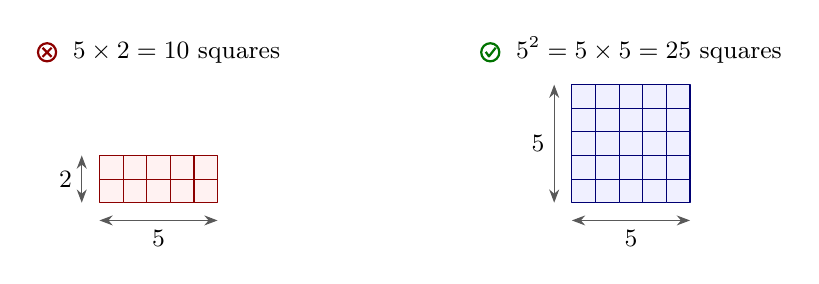
\begin{tikzpicture}[scale=0.3,line join=round]
  \foreach \x in {0,...,4} \foreach \y in {0,1}
    \draw[red!55!black,fill=red!5] (\x,\y) rectangle ++(1,1);
  \draw[<->,>=Stealth,gray!70!black] (0,-0.75) -- (5,-0.75)
    node[midway,below,font=\small,black] {$5$};
  \draw[<->,>=Stealth,gray!70!black] (-0.75,0) -- (-0.75,2)
    node[midway,left,font=\small,black] {$2$};
  \node[font=\small,anchor=south] at (2.5,5.5)
    {\crossmark\; $5\times2=10$ squares};
  \begin{scope}[xshift=20cm]
    \foreach \x in {0,...,4} \foreach \y in {0,...,4}
      \draw[blue!45!black,fill=blue!6] (\x,\y) rectangle ++(1,1);
    \draw[<->,>=Stealth,gray!70!black] (0,-0.75) -- (5,-0.75)
      node[midway,below,font=\small,black] {$5$};
    \draw[<->,>=Stealth,gray!70!black] (-0.75,0) -- (-0.75,5)
      node[midway,left,font=\small,black] {$5$};
    \node[font=\small,anchor=south] at (2.5,5.5)
      {\tickmark\; $5^2=5\times5=25$ squares};
  \end{scope}
\end{tikzpicture}}

% A root drawn as the arrow that returns to the number the index started
% from. The second commonest error is to undo an index by dividing by it,
% and a return arrow labelled with a question rather than an operation
% shows that the root is a search for the number that rebuilds the total.
% \undoloop{<start>}{<result>}{<forward label>}{<return label>}
\newcommand{\undoloop}[4]{%
\begin{tikzpicture}[baseline=(a.base),
    nd/.style={draw,rounded corners=3pt,thick,minimum width=0.95cm,
      minimum height=0.7cm,font=\small}]
  \node[nd,draw=blue!45!black,fill=blue!6] (a) at (0,0) {#1};
  \node[nd,draw=orange!60!black,fill=orange!6] (b) at (4.3,0) {#2};
  \draw[->,>=Stealth,thick,blue!45!black] (a) to[bend left=26]
    node[midway,above,font=\scriptsize,black] {#3} (b);
  \draw[->,>=Stealth,thick,densely dashed,orange!60!black] (b) to[bend left=26]
    node[midway,below,font=\scriptsize,black] {#4} (a);
\end{tikzpicture}}

% A cancelled factor, with the 1 it leaves behind written above it. The
% strongest misconception about cancelling is that a crossed-out factor
% leaves an empty place, and that an empty place is worth nothing.
\newcommand{\cancelone}[1]{\overset{\textcolor{green!45!black}{1}}{\cancel{#1}}}

% The pairing that cancelling does, drawn as arcs from a factor on the
% top to the one factor on the bottom that it is divided out with. The
% two 3s sit in different columns on purpose, so that the pair is read by
% value and not by position.
\newcommand{\pairarcs}{%
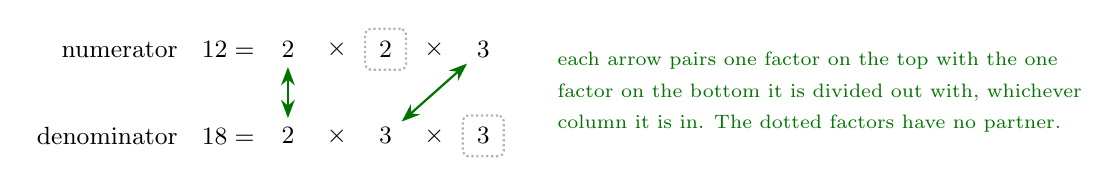
\begin{tikzpicture}[font=\small,baseline=(current bounding box.center)]
  \node[anchor=east] at (-0.3,0.55) {numerator \; $12=$};
  \node[anchor=east] at (-0.3,-0.55) {denominator \; $18=$};
  \node (n1) at (0,0.55) {$2$};   \node at (0.62,0.55) {$\times$};
  \node (n2) at (1.24,0.55) {$2$}; \node at (1.86,0.55) {$\times$};
  \node (n3) at (2.48,0.55) {$3$};
  \node (d1) at (0,-0.55) {$2$};   \node at (0.62,-0.55) {$\times$};
  \node (d2) at (1.24,-0.55) {$3$}; \node at (1.86,-0.55) {$\times$};
  \node (d3) at (2.48,-0.55) {$3$};
  \draw[green!45!black,thick,<->,>=Stealth] (n1) -- (d1);
  \draw[green!45!black,thick,<->,>=Stealth] (n3) -- (d2);
  \node[draw=gray!60,densely dotted,thick,rounded corners=2pt,
    minimum size=0.52cm,inner sep=1pt] at (n2) {};
  \node[draw=gray!60,densely dotted,thick,rounded corners=2pt,
    minimum size=0.52cm,inner sep=1pt] at (d3) {};
  \node[font=\scriptsize,text=green!45!black,anchor=west] at (3.3,0.4)
    {each arrow pairs one factor on the top with the one};
  \node[font=\scriptsize,text=green!45!black,anchor=west] at (3.3,0.0)
    {factor on the bottom it is divided out with, whichever};
  \node[font=\scriptsize,text=green!45!black,anchor=west] at (3.3,-0.4)
    {column it is in. The dotted factors have no partner.};
\end{tikzpicture}}

% The factors of a term drawn as tiles, one tile per factor, with the
% number tiles and the variable tiles coloured differently. The index
% then counts tiles of one colour only, so a coefficient cannot be swept
% into it, and the wrong reading is one tile too long.
% \factortiles{<number>}{<variable>}{<the number squared>}
\newcommand{\factortiles}[3]{%
\begin{tikzpicture}[font=\small,
   nt/.style={draw=orange!60!black,fill=orange!6,rounded corners=2pt,thick,
     minimum size=0.72cm,inner sep=1pt},
   vt/.style={draw=blue!45!black,fill=blue!6,rounded corners=2pt,thick,
     minimum size=0.72cm,inner sep=1pt},
   wt/.style={draw=red!55!black,fill=red!5,rounded corners=2pt,thick,
     minimum size=0.72cm,inner sep=1pt}]
  % the correct reading
  \node[nt] at (0,0) {$#1$};
  \node[vt] at (0.85,0) {$#2$};
  \node[vt] at (1.7,0) {$#2$};
  \node[anchor=west] at (2.25,0) {$=#1#2^2$};
  \node[anchor=west] at (3.4,0) {\tickmark};
  \draw[decorate,decoration={brace,amplitude=4pt,mirror},blue!45!black]
    (0.45,-0.45) -- (2.1,-0.45);
  \node[font=\scriptsize,text=blue!45!black,anchor=north] at (1.28,-0.62)
    {two $#2$ tiles, so $#2^2$};
  \draw[->,>=Stealth,orange!60!black] (0,0.72) -- (0,0.42);
  \node[font=\scriptsize,text=orange!60!black,anchor=south] at (0,0.74)
    {the $#1$ multiplies, it is not a $#2$};
  % the wrong reading, one tile too long
  \begin{scope}[yshift=-2.3cm]
    \node[wt] at (0,0) {$#1$};   \node[wt] at (0.85,0) {$#2$};
    \node[wt] at (1.7,0) {$#1$}; \node[wt] at (2.55,0) {$#2$};
    \node[anchor=west] at (3.1,0) {$=#1#2\times#1#2=#3#2^2$};
    \node[anchor=west] at (6.3,0) {\crossmark};
    \draw[decorate,decoration={brace,amplitude=4pt,mirror},red!55!black]
      (-0.4,-0.45) -- (2.95,-0.45);
    \node[font=\scriptsize,text=red!55!black,anchor=north] at (1.28,-0.62)
      {four tiles, so this is not $#1#2^2$};
  \end{scope}
\end{tikzpicture}}

% The sign of a power of a negative number, drawn by pairing the minus
% signs off. An even index pairs them all and an odd index always leaves
% one over, so the sign becomes something counted rather than sensed.
\newcommand{\signpairs}{%
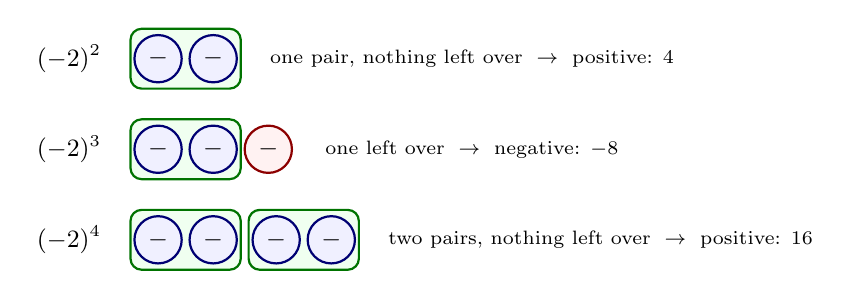
\begin{tikzpicture}[font=\small,
   tok/.style={circle,draw=blue!45!black,fill=blue!6,thick,
     minimum size=0.6cm,inner sep=0pt,font=\small},
   odd/.style={circle,draw=red!55!black,fill=red!5,thick,
     minimum size=0.6cm,inner sep=0pt,font=\small},
   pr/.style={rounded corners=4pt,draw=green!45!black,fill=green!6,thick}]
  % (-2)^2
  \node[anchor=east] at (-0.2,0) {$(-2)^2$};
  \filldraw[pr] (0.05,-0.38) rectangle (1.45,0.38);
  \node[tok] at (0.4,0) {$-$}; \node[tok] at (1.1,0) {$-$};
  \node[anchor=west,font=\scriptsize] at (1.7,0)
    {one pair, nothing left over \;$\rightarrow$\; positive: $4$};
  % (-2)^3
  \node[anchor=east] at (-0.2,-1.15) {$(-2)^3$};
  \filldraw[pr] (0.05,-1.53) rectangle (1.45,-0.77);
  \node[tok] at (0.4,-1.15) {$-$}; \node[tok] at (1.1,-1.15) {$-$};
  \node[odd] at (1.8,-1.15) {$-$};
  \node[anchor=west,font=\scriptsize] at (2.4,-1.15)
    {one left over \;$\rightarrow$\; negative: $-8$};
  % (-2)^4
  \node[anchor=east] at (-0.2,-2.3) {$(-2)^4$};
  \filldraw[pr] (0.05,-2.68) rectangle (1.45,-1.92);
  \filldraw[pr] (1.55,-2.68) rectangle (2.95,-1.92);
  \node[tok] at (0.4,-2.3) {$-$}; \node[tok] at (1.1,-2.3) {$-$};
  \node[tok] at (1.9,-2.3) {$-$}; \node[tok] at (2.6,-2.3) {$-$};
  \node[anchor=west,font=\scriptsize] at (3.2,-2.3)
    {two pairs, nothing left over \;$\rightarrow$\; positive: $16$};
\end{tikzpicture}}

\begin{document}

\begin{center}
  {\Large\bfseries An Introduction to Indices and Roots}\\[3pt]
  {\large Worked Solutions}
\end{center}

Each solution is written out using the method taught in the worked example that
comes before the question on the worksheet, and in the same steps.

\begin{keyidea}
An \textbf{index} tells us how many times a number is multiplied by itself. In
$5^3$ the number $5$ is called the \textbf{base} and the small raised number
$3$ is called the \textbf{index}, so $5^3$ means $5\times5\times5$. The plural
of index is \textbf{indices}. A \textbf{root} undoes an index.
\end{keyidea}

\begin{notation}{indices and roots}
\renewcommand{\arraystretch}{1.4}%
\begin{tabular}{@{}>{\large}p{4.3cm}@{\hspace{0.8em}}p{5.0cm}@{\hspace{0.8em}}l@{}}
$a^2=a\times a$ & ``$a$ squared'' & for example \; $7^2=7\times7=49$\\
$a^3=a\times a\times a$ & ``$a$ cubed'' & for example \; $2^3=2\times2\times2=8$\\
$\sqrt{a}$ & the square root of $a$ & for example \; $\sqrt{49}=7$\\
$\sqrt[3]{a}$ & the cube root of $a$ & for example \; $\sqrt[3]{8}=2$\\
\end{tabular}
\end{notation}

\parttitle{1}{Indices and roots of numbers}

\qhead{1}{Work out each calculation and join it to its answer.}
\wsol
An index is worked out by writing the multiplication out in full. A root is
worked out by finding the number that gives the answer when it is multiplied by
itself the right number of times.

\vspace{2pt}
\begin{center}
\renewcommand{\arraystretch}{1.45}
\begin{tabular}{|c|l|c|}
\hline
\textbf{Number} & \textbf{Calculation} & \textbf{Joins to}\\
\hline
$1$ & $5^2=5\times5=25$ & D\\ \hline
$2$ & $\sqrt{100}=10$, because $10\times10=100$ & H\\ \hline
$3$ & $2^3=2\times2\times2=8$ & B\\ \hline
$4$ & $0.2^2=0.2\times0.2=0.04$ & F\\ \hline
$5$ & $\sqrt{0.25}=0.5$, because $0.5\times0.5=0.25$ & A\\ \hline
$6$ & $10^3=10\times10\times10=1000$ & E\\ \hline
$7$ & $\sqrt[3]{8}=2$, because $2\times2\times2=8$ & C\\ \hline
$8$ & $1.5^2=1.5\times1.5=2.25$ & G\\ \hline
\end{tabular}
\end{center}

In numbers $4$ and $8$ the base is a decimal. We multiply the digits first and
then count the decimal places. For number $4$ we have $2\times2=4$, and $0.2$
has one decimal place and $0.2$ has one decimal place, so the answer has two
decimal places, which gives $0.04$. For number $8$ we have $15\times15=225$,
and again there are two decimal places altogether, which gives $2.25$.

\vspace{2pt}
The joins are $1$--D, $2$--H, $3$--B, $4$--F, $5$--A, $6$--E, $7$--C and
$8$--G.

\begin{mistake}{reading the index as a multiplier}
The index is \textbf{not} a second number to multiply by, so $5^2$ is not
$5\times2=10$. In $5^2$ the index $2$ says how many $5$s are multiplied together.
In Q2 this mistake gives $6^2=12$ m$^2$ and $4^3=12$ cm$^3$. Counting the
squares in each picture shows the difference.

\vspace{2pt}
\begin{center}
\indexarrays
\end{center}
\end{mistake}

\qhead{2}{Area, side, volume and edge.}
\wsol
\begin{enumerate}
\item The patio is a square with sides of length $6$ m, so its area is the
length of a side multiplied by itself.
\[\text{Area}=6^2=6\times6=36\text{ m}^2\]

\item The area of the second patio is $144$ m$^2$, so the length of a side is
the number that gives $144$ when it is multiplied by itself. That number is the
square root of $144$.
\[\text{Side}=\sqrt{144}=12\text{ m},\qquad\text{because }12\times12=144\]

\item The box is a cube with edges of length $4$ cm, so its volume is the
length of an edge multiplied by itself three times.
\[\text{Volume}=4^3=4\times4\times4=64\text{ cm}^3\]

\item The volume of the second box is $125$ cm$^3$, so the length of an edge is
the number that gives $125$ when three of them are multiplied together. That
number is the cube root of $125$.
\[\text{Edge}=\sqrt[3]{125}=5\text{ cm},\qquad\text{because }5\times5\times5=125\]

\item The area of the floor tile is $0.25$ m$^2$, so the length of a side is the
number that gives $0.25$ when it is multiplied by itself. That number is the
square root of $0.25$.
\[\text{Side}=\sqrt{0.25}=0.5\text{ m},\qquad\text{because }0.5\times0.5=0.25\]

\item The square numbers either side of $50$ are $7^2=49$ and $8^2=64$. The area
of $50$ m$^2$ is between $49$ and $64$, so the length of a side is between
$\sqrt{49}=7$ m and $\sqrt{64}=8$ m.
\[7^2=49\;<\;50\;<\;64=8^2,\qquad\text{so the side is between }7\text{ m and }8\text{ m.}\]
Because $50$ is much closer to $49$ than to $64$, the side is only a little more
than $7$ m. On a calculator $\sqrt{50}=7.07\ldots$ m, which checks the answer.
\end{enumerate}

\begin{mistake}{dividing by the index to find a root}
A root undoes an index, but it does \textbf{not} divide by the index. The
square root of $144$ is not $144\div2=72$, and the cube root of $125$ is not
$125\div3$. A root asks which number, multiplied by itself the right number of
times, rebuilds the number we started with. An answer is checked by multiplying
it back: $72\times72=5184$, which is not $144$, but $12\times12=144$.

\vspace{4pt}
\begin{center}
\undoloop{$3$}{$9$}{square it: $3\times3$}{$\sqrt{9}$: what, times itself, makes $9$?}
\hfill
\undoloop{$2$}{$8$}{cube it: $2\times2\times2$}{$\sqrt[3]{8}$: what, three times, makes $8$?}
\end{center}
\end{mistake}

\parttitle{2}{Indices and algebraic variables}

\qhead{3}{Write each expression in index form.}
\wsol
We count how many times each algebraic variable appears in the numerator and
how many times it appears in the denominator, and we write each count as an
index.

\begin{enumerate}
\item The variable $a$ appears $4$ times, so $a\times a\times a\times a=a^4$.

\item We use the three steps of the worked example.

\vspace{2pt}
\renewcommand{\arraystretch}{1.5}
\begin{tabular}{@{}l@{\hspace{1.2em}}l@{}}
\textbf{Step 1 --- count the numerator.}
  & $c$ appears $3$ times, so the numerator is $c^3$.\\
\textbf{Step 2 --- count the denominator.}
  & $d$ appears $2$ times, so the denominator is $d^2$.\\
\textbf{Step 3 --- write the fraction.}
  & $\dfrac{c\times c\times c}{d\times d}=\dfrac{c^3}{d^2}$\\
\end{tabular}

\item The variable $b$ appears $5$ times, so
$b\times b\times b\times b\times b=b^5$.

\item The number $3$ multiplies the variable, so it is written in front, and
$m$ appears $2$ times, which gives $3\times m\times m=3m^2$ (remember
$3m^2=3\times m\times m$).

\item The numerator has $p$ appearing $3$ times and the denominator has $q$
appearing $4$ times, so
$\dfrac{p\times p\times p}{q\times q\times q\times q}=\dfrac{p^3}{q^4}$.

\item The numerator is $2\times x\times x\times x=2x^3$ and the denominator is
$y\times y=y^2$, so
$\dfrac{2\times x\times x\times x}{y\times y}=\dfrac{2x^3}{y^2}$.

\item The numerator has two different variables in it, and each one is counted
separately: $a$ appears $2$ times and $b$ appears $3$ times, so the numerator
is $a^2b^3$. The denominator is $c^2$, which gives
$\dfrac{a\times a\times b\times b\times b}{c\times c}=\dfrac{a^2b^3}{c^2}$.

\item The numerator is $t\times t=t^2$ and the denominator is
$5\times u\times u\times u=5u^3$, so
$\dfrac{t\times t}{5\times u\times u\times u}=\dfrac{t^2}{5u^3}$.
\end{enumerate}

\newpage

\qhead{4}{Write each expression out in full as a multiplication.}
\wsol
The index tells us how many times the base is written down in the
multiplication.

\begin{enumerate}
\item $x^3=x\times x\times x$, which is given on the worksheet.

\item The index is $5$ and the base is $y$, so
$y^5=y\times y\times y\times y\times y$.

\item The index belongs to the $t$ only, and the $4$ multiplies the whole of
$t^2$, so $4t^2=4\times t\times t$.

\item The numerator is $m^2=m\times m$ and the denominator is
$n^3=n\times n\times n$, so
$\dfrac{m^2}{n^3}=\dfrac{m\times m}{n\times n\times n}$.

\item The numerator is $a^4=a\times a\times a\times a$. The denominator is $b$,
which has an index of $1$ that is not written, so $b$ appears once and
$\dfrac{a^4}{b}=\dfrac{a\times a\times a\times a}{b}$.
\end{enumerate}

\begin{mistake}{counting the number in front as part of the index}
In Q4(c) the index belongs to the $t$ only, so $4t^2=4\times t\times t$. It is
\textbf{not} $4t\times4t$. If $t=3$ then $4t^2=4\times3\times3=36$, but
$4t\times4t=12\times12=144$. In the same way, in Q3(d) $3\times m\times m$ is
$3m^2$ and not $m^3$, because the index counts only the factors that are $m$.
Each factor below is one tile, and the index counts only the tiles that hold the
variable.

\vspace{4pt}
\begin{center}
\factortiles{4}{t}{16}
\end{center}
\end{mistake}

\parttitle{3}{Cancelling factors in a fraction}

The \textbf{numerator} is the expression on the top of a fraction and the
\textbf{denominator} is the expression on the bottom. A factor that appears in
both is divided out of both, which is called cancelling.

\begin{wex}{simplify $\dfrac{12}{18}$}
\small
\renewcommand{\arraystretch}{1.9}
\begin{tabular}{@{}l@{\hspace{1.2em}}l@{}}
\textbf{Step 1 --- write the numerator and the denominator as multiplications.}
  & $\dfrac{12}{18}=\dfrac{2\times2\times3}{2\times3\times3}$\\
\textbf{Step 2 --- cross out each factor that appears in both.}
  & $\dfrac{12}{18}=\dfrac{\cancel{2}\times2\times\cancel{3}}
    {\cancel{2}\times\cancel{3}\times3}$\\
\textbf{Step 3 --- multiply what is left on the top and on the bottom.}
  & $\dfrac{12}{18}=\dfrac{2}{3}$\\
\end{tabular}
\end{wex}

\begin{mistake}{cancelling by column, or cancelling digits}
Cancelling pairs \textbf{one} factor on the top with \textbf{one} factor on
the bottom that has the same value, whichever column each of them is in. The
pairs are not found by lining the columns up, and one factor cannot cancel two.
Digits are not factors either: in $14/21$ the two $1$s cannot be crossed out,
because $14=7\times2$ and $21=7\times3$, so the factor they share is $7$.

\vspace{4pt}
\begin{center}
\pairarcs
\end{center}
\end{mistake}

\qhead{5}{Simplify each fraction by cancelling.}
\wsol
Each numerator and each denominator is written as a multiplication of its
factors first, so that the factors they share can be seen and crossed out.

\begin{enumerate}
\item $8=2\times2\times2$ and $12=2\times2\times3$, and the factors $2$ and $2$
appear in both.
\[\frac{8}{12}=\frac{2\times2\times2}{2\times2\times3}
  =\frac{\cancel{2}\times\cancel{2}\times2}{\cancel{2}\times\cancel{2}\times3}
  =\frac{2}{3}\]

\item $15=5\times3$ and $25=5\times5$, and the factor $5$ appears in both.
\[\frac{15}{25}=\frac{5\times3}{5\times5}
  =\frac{\cancel{5}\times3}{\cancel{5}\times5}=\frac{3}{5}\]

\item $18=2\times3\times3$ and $24=2\times3\times2\times2$, and the factors $2$
and $3$ appear in both.
\[\frac{18}{24}=\frac{2\times3\times3}{2\times3\times2\times2}
  =\frac{\cancel{2}\times\cancel{3}\times3}
   {\cancel{2}\times\cancel{3}\times2\times2}=\frac{3}{4}\]

\item $14=7\times2$ and $21=7\times3$, and the factor $7$ appears in both.
\[\frac{14}{21}=\frac{7\times2}{7\times3}
  =\frac{\cancel{7}\times2}{\cancel{7}\times3}=\frac{2}{3}\]

\item $45=5\times3\times3$ and $60=5\times3\times2\times2$, and the factors $5$
and $3$ appear in both.
\[\frac{45}{60}=\frac{5\times3\times3}{5\times3\times2\times2}
  =\frac{\cancel{5}\times\cancel{3}\times3}
   {\cancel{5}\times\cancel{3}\times2\times2}=\frac{3}{4}\]

\item $24=2\times2\times2\times3$ and $36=2\times2\times3\times3$, and the
factors $2$, $2$ and $3$ appear in both.
\[\frac{24}{36}=\frac{2\times2\times2\times3}{2\times2\times3\times3}
  =\frac{\cancel{2}\times\cancel{2}\times2\times\cancel{3}}
   {\cancel{2}\times\cancel{2}\times\cancel{3}\times3}=\frac{2}{3}\]

\item $12$ of the $28$ pupils walk, so the fraction of the class who walk is
$\dfrac{12}{28}$. Here $12=2\times2\times3$ and $28=2\times2\times7$, and the
factors $2$ and $2$ appear in both.
\[\frac{12}{28}=\frac{2\times2\times3}{2\times2\times7}
  =\frac{\cancel{2}\times\cancel{2}\times3}{\cancel{2}\times\cancel{2}\times7}
  =\frac{3}{7}\]

\item $45$ g of the $120$ g is sugar, so the fraction that is sugar is
$\dfrac{45}{120}$. Here $45=3\times3\times5$ and $120=2\times2\times2\times3\times5$,
and the factors $3$ and $5$ appear in both.
\[\frac{45}{120}=\frac{3\times3\times5}{2\times2\times2\times3\times5}
  =\frac{3\times\cancel{3}\times\cancel{5}}
   {2\times2\times2\times\cancel{3}\times\cancel{5}}
  =\frac{3}{2\times2\times2}=\frac{3}{8}\]
\end{enumerate}

\newpage

\qhead{6}{Simplify each fraction by cancelling, then write the answer in index
form.}
\wsol
The numbers and the variables are cancelled separately. Where every factor on
the bottom is crossed out, the denominator is written as $1$ before the
fraction is written as its numerator.

\begin{enumerate}
\item Two of the four $a$s on the top cancel with the two $a$s on the bottom,
and two $a$s are left on the top.
\[\frac{a\times a\times a\times a}{a\times a}
  =\frac{\cancel{a}\times\cancel{a}\times a\times a}{\cancel{a}\times\cancel{a}}
  =\frac{a\times a}{1}=a^2\]

\item Two of the five $b$s on the top cancel with the two $b$s on the bottom,
and three $b$s are left on the top.
\[\frac{b\times b\times b\times b\times b}{b\times b}
  =\frac{\cancel{b}\times\cancel{b}\times b\times b\times b}
   {\cancel{b}\times\cancel{b}}=\frac{b\times b\times b}{1}=b^3\]

\item One factor of $2$ and one factor of $m$ cancel.
\[\frac{2\times2\times m\times m}{2\times m}
  =\frac{\cancel{2}\times2\times\cancel{m}\times m}{\cancel{2}\times\cancel{m}}
  =\frac{2\times m}{1}=2m\]

\item The factor $5$ appears on the top and on the bottom, so it cancels, but
the factor $3$ appears on the top only, so it stays. One factor of $p$ cancels
as well.
\[\frac{3\times5\times p\times p\times p}{5\times p}
  =\frac{3\times\cancel{5}\times\cancel{p}\times p\times p}
   {\cancel{5}\times\cancel{p}}=\frac{3\times p\times p}{1}=3p^2\]

\item One factor of $x$ and one factor of $y$ cancel. Here a factor of $y$ is
left on the bottom, so the denominator is $y$ and not $1$.
\[\frac{x\times x\times y}{x\times y\times y}
  =\frac{\cancel{x}\times x\times\cancel{y}}
   {\cancel{x}\times\cancel{y}\times y}=\frac{x}{y}\]

\item One factor of $3$ and one factor of $t$ cancel, and a factor of $3$ is
left on the bottom.
\[\frac{2\times3\times t\times t}{3\times3\times t}
  =\frac{2\times\cancel{3}\times\cancel{t}\times t}
   {\cancel{3}\times3\times\cancel{t}}=\frac{2\times t}{3}=\frac{2t}{3}\]

\item Here $4=2\times2$ and $6=2\times3$, so one factor of $2$ cancels. One
factor of $x$ and one factor of $y$ cancel as well.
\[\frac{4\times x\times x\times y}{6\times x\times y\times y}
  =\frac{\cancel{2}\times2\times\cancel{x}\times x\times\cancel{y}}
   {\cancel{2}\times3\times\cancel{x}\times\cancel{y}\times y}
  =\frac{2\times x}{3\times y}=\frac{2x}{3y}\]

\item One factor of $5$, one factor of $a$ and one factor of $b$ cancel. A
factor of $a$ is left on the bottom, so the denominator is $a$ and not $1$.
\[\frac{5\times5\times a\times b\times b}{5\times a\times a\times b}
  =\frac{\cancel{5}\times5\times\cancel{a}\times\cancel{b}\times b}
   {\cancel{5}\times\cancel{a}\times a\times\cancel{b}}
  =\frac{5\times b}{a}=\frac{5b}{a}\]

\item
\modelans
Two factors of $a$ cancel from the top and from the bottom. Every factor on the
top has cancelled, so the numerator is $1$, and one factor of $a$ is left on the
bottom. Lena has put the $a$ that is left on the top instead of on the bottom.
The correct answer is $\dfrac{1}{a}$.
\[\frac{a\times a}{a\times a\times a}
  =\frac{\cancel{a}\times\cancel{a}}{\cancel{a}\times\cancel{a}\times a}
  =\frac{1}{a}\]
\alsoacc
An answer that shows the mistake by substituting a number is also correct. For
example $a=2$ gives $\dfrac{2\times2}{2\times2\times2}=\dfrac{4}{8}=\dfrac{1}{2}$,
which is $\dfrac{1}{a}$ and not $a$.
\end{enumerate}

\newpage

\parttitle{4}{Simplifying fractions written with indices}

Each power is written out in full as a multiplication, the factors that appear
on the top and on the bottom are cancelled, and what is left is written in
index form.

\qhead{7}{Simplify each fraction and join it to its answer.}
\wsol
\begin{enumerate}[label=\textbf{\arabic*.}, leftmargin=*, itemsep=7pt]
\item Two of the five $a$s cancel, leaving three.
$\dfrac{a^5}{a^2}
  =\dfrac{\cancel{a}\times\cancel{a}\times a\times a\times a}
   {\cancel{a}\times\cancel{a}}=\dfrac{a\times a\times a}{1}=a^3$, which joins
to \textbf{D}.

\item Every factor on the top and on the bottom cancels, so the numerator is
$1$ and the denominator is $1$.
$\dfrac{a^2}{a^2}=\dfrac{\cancel{a}\times\cancel{a}}{\cancel{a}\times\cancel{a}}
  =\dfrac{1}{1}=1$, which joins to \textbf{F}.

\item Here $6=2\times3$, so a factor of $2$ cancels as well as two of the $a$s.
$\dfrac{6a^4}{2a^2}
  =\dfrac{\cancel{2}\times3\times\cancel{a}\times\cancel{a}\times a\times a}
   {\cancel{2}\times\cancel{a}\times\cancel{a}}
  =\dfrac{3\times a\times a}{1}=3a^2$, which joins to \textbf{H}.

\item One factor of $a$ and the single factor of $b$ cancel.
$\dfrac{a^3b}{ab}
  =\dfrac{\cancel{a}\times a\times a\times\cancel{b}}{\cancel{a}\times\cancel{b}}
  =\dfrac{a\times a}{1}=a^2$, which joins to \textbf{G}.

\item Here $4=2\times2$ and $8=2\times2\times2$, so two factors of $2$ cancel
and one factor of $2$ is left on the bottom.
$\dfrac{4a^2}{8a}
  =\dfrac{\cancel{2}\times\cancel{2}\times\cancel{a}\times a}
   {\cancel{2}\times\cancel{2}\times2\times\cancel{a}}=\dfrac{a}{2}$, which
joins to \textbf{E}.

\item Both factors of $a$ cancel, and one of the three $b$s cancels.
$\dfrac{a^2b^3}{a^2b}
  =\dfrac{\cancel{a}\times\cancel{a}\times\cancel{b}\times b\times b}
   {\cancel{a}\times\cancel{a}\times\cancel{b}}=\dfrac{b\times b}{1}=b^2$,
which joins to \textbf{A}.

\item Here $10=5\times2$, so the factor $5$ cancels and all three $a$s cancel.
$\dfrac{10a^3}{5a^3}
  =\dfrac{\cancel{5}\times2\times\cancel{a}\times\cancel{a}\times\cancel{a}}
   {\cancel{5}\times\cancel{a}\times\cancel{a}\times\cancel{a}}
  =\dfrac{2}{1}=2$, which joins to \textbf{C}.

\item Two of the six $a$s cancel, leaving four.
$\dfrac{a^6}{a^2}
  =\dfrac{\cancel{a}\times\cancel{a}\times a\times a\times a\times a}
   {\cancel{a}\times\cancel{a}}=\dfrac{a\times a\times a\times a}{1}=a^4$,
which joins to \textbf{B}.
\end{enumerate}

\vspace{4pt}
The joins are $1$--D, $2$--F, $3$--H, $4$--G, $5$--E, $6$--A, $7$--C and
$8$--B.

\newpage

\qhead{8}{Writing fractions that simplify to a given expression.}
\begin{enumerate}
\item
\modelans
Three fractions that simplify to $2a^2$ are $\dfrac{2a^3}{a}$, \;
$\dfrac{4a^3}{2a}$ \; and \; $\dfrac{6a^5}{3a^3}$. The second and the third
both have a number other than $1$ in the denominator. Each one is checked by
cancelling.
\begin{align*}
\frac{2a^3}{a}&=\frac{2\times\cancel{a}\times a\times a}{\cancel{a}}
  =\frac{2\times a\times a}{1}=2a^2\\[2pt]
\frac{4a^3}{2a}&=\frac{\cancel{2}\times2\times\cancel{a}\times a\times a}
  {\cancel{2}\times\cancel{a}}=\frac{2\times a\times a}{1}=2a^2\\[2pt]
\frac{6a^5}{3a^3}&=\frac{\cancel{3}\times2\times\cancel{a}\times\cancel{a}
  \times\cancel{a}\times a\times a}
  {\cancel{3}\times\cancel{a}\times\cancel{a}\times\cancel{a}}
  =\frac{2\times a\times a}{1}=2a^2
\end{align*}
\alsoacc
Any fraction whose numerator is its denominator multiplied by $2a^2$ is
correct, for example $\dfrac{10a^4}{5a^2}$, $\dfrac{2a^4}{a^2}$ or
$\dfrac{8a^3}{4a}$. One of the three fractions must have a number other than
$1$ in its denominator.

\item
\modelans
One fraction that simplifies to $\dfrac{a^2}{b}$ is $\dfrac{a^3}{ab}$, because
one factor of $a$ cancels from the top and from the bottom.
\[\frac{a^3}{ab}
  =\frac{\cancel{a}\times a\times a}{\cancel{a}\times b}=\frac{a^2}{b}\]
\alsoacc
Any fraction whose numerator has exactly two more factors of $a$ than its
denominator, and whose denominator has exactly one more factor of $b$ than its
numerator, is correct, as long as it is not $\dfrac{a^2}{b}$ itself. Examples are $\dfrac{a^2b}{b^2}$, $\dfrac{a^4}{a^2b}$
and $\dfrac{a^4b}{a^2b^2}$.

\item
\modelans
One fraction that uses $x$, $y$ and $z$ and simplifies to $\dfrac{1}{xy^2}$ is
$\dfrac{z}{xy^2z}$. The factor $z$ cancels from the top and from the bottom,
which leaves $1$ on the top.
\[\frac{z}{xy^2z}=\frac{\cancel{z}}{x\times y\times y\times\cancel{z}}
  =\frac{1}{xy^2}\]
\alsoacc
Any fraction in which every factor on the top also appears on the bottom, and
the factors left on the bottom are one $x$ and two $y$s, is correct. Examples
are $\dfrac{xz}{x^2y^2z}$ and $\dfrac{yz^2}{xy^3z^2}$.

\item
\modelans
Ben has crossed out every factor correctly, but he has then written that
nothing is left. Cancelling divides the numerator and the denominator by the
same factor, and a factor divided by itself is $1$, not $0$. When every factor
on the top cancels the numerator is $1$, and when every factor on the bottom
cancels the denominator is $1$, so the correct answer is $\dfrac{1}{1}=1$.
\[\frac{3a^2}{3a^2}
  =\frac{\cancel{3}\times\cancel{a}\times\cancel{a}}
   {\cancel{3}\times\cancel{a}\times\cancel{a}}=\frac{1}{1}=1\]
\alsoacc
Any answer that says a number or a variable divided by itself is $1$, and that
gives the correct answer of $1$, is correct. An answer that checks the result
by substituting a number, for example $a=2$ giving
$\dfrac{3\times2\times2}{3\times2\times2}=\dfrac{12}{12}=1$, is also correct.
\end{enumerate}

\begin{mistake}{a crossed-out factor leaves nothing}
Crossing a factor out does not rub it off the page. A factor divided by itself
is $1$, so a crossed-out factor leaves a $1$ behind. It never leaves nothing,
and it never leaves a $0$.
\[\frac{12}{18}
  =\frac{\cancelone{2}\times2\times\cancelone{3}}
        {\cancelone{2}\times\cancelone{3}\times3}
  =\frac{1\times2\times1}{1\times1\times3}=\frac{2}{3}
  \qquad\qquad
  \frac{a^2}{a^2}
  =\frac{\cancelone{a}\times\cancelone{a}}{\cancelone{a}\times\cancelone{a}}
  =\frac{1\times1}{1\times1}=\frac{1}{1}=1\]
\end{mistake}

\qhead{9}{A quicker way to simplify a fraction such as $\dfrac{a^7}{a^3}$.}
\begin{enumerate}
\item
\wsol
Each power is written out in full, and the factors that appear on the top and
on the bottom are cancelled.
\[\frac{a^7}{a^3}
  =\frac{\cancel{a}\times\cancel{a}\times\cancel{a}\times a\times a\times a\times a}
   {\cancel{a}\times\cancel{a}\times\cancel{a}}
  =\frac{a\times a\times a\times a}{1}=a^4\]
In the same way, four of the nine $b$s cancel, leaving five, so
$\dfrac{b^9}{b^4}=b^5$. Five of the six $c$s cancel, leaving one, so
$\dfrac{c^6}{c^5}=c^1=c$.

\item
\modelans
Subtract the index on the bottom from the index on the top, and keep the same
base. For example $7-3=4$, so $\dfrac{a^7}{a^3}=a^4$. This works because each
factor on the bottom cancels one factor on the top, so the number of factors
left on the top is the index on the top take away the index on the bottom.
\alsoacc
Any answer that describes taking the index on the bottom away from the index on
the top is correct.

\item
\wsol
\[\frac{x^{20}}{x^{13}}=x^{20-13}=x^7\qquad\qquad
  \frac{y^{100}}{y^{99}}=y^{100-99}=y^1=y\]

\item
\wsol
The quicker way gives $\dfrac{a^3}{a^3}=a^{3-3}=a^0$. Cancelling gives
\[\frac{a^3}{a^3}
  =\frac{\cancel{a}\times\cancel{a}\times\cancel{a}}
   {\cancel{a}\times\cancel{a}\times\cancel{a}}=\frac{1}{1}=1\]
Both ways simplify the same fraction, so they must give the same answer. This
suggests that $a^0=1$.
\end{enumerate}

\newpage

\parttitle{5}{Extension: factorials, negative numbers and the fourth dimension}

The \textbf{factorial} $n!$ means multiply together every whole number from $n$
down to $1$.

\qhead{10}{Work out each factorial.}
\wsol
\begin{enumerate}
\item $3!=3\times2\times1=6$
\item $4!=4\times3\times2\times1=24$
\item $6!=6\times5\times4\times3\times2\times1=720$
\item $1!=1$, because the only whole number from $1$ down to $1$ is $1$ itself.
\end{enumerate}

\begin{wex}{simplify $\dfrac{6!}{4!}$}
\small
Both factorials are written out in full. Every whole number from $4$ downwards
appears on the top and on the bottom, so all of those factors cancel.

\smallskip
\[\frac{6!}{4!}
  =\frac{6\times5\times\cancel{4}\times\cancel{3}\times\cancel{2}\times\cancel{1}}
   {\cancel{4}\times\cancel{3}\times\cancel{2}\times\cancel{1}}
  =\frac{6\times5}{1}=6\times5=30\]
\end{wex}

\qhead{11}{Simplify each expression by writing the factorials out in full and
cancelling.}
\wsol
The factorials are not worked out first. Every factor that appears on the top
and on the bottom is crossed out, and what is left is multiplied.

\begin{enumerate}
\item Every whole number from $3$ downwards appears on the top and on the
bottom, so all of those factors cancel and the denominator is $1$.
\[\frac{5!}{3!}
  =\frac{5\times4\times\cancel{3}\times\cancel{2}\times\cancel{1}}
   {\cancel{3}\times\cancel{2}\times\cancel{1}}
  =\frac{5\times4}{1}=5\times4=20\]

\item Every whole number from $9$ downwards cancels, and only the $10$ is left
on the top.
\[\frac{10!}{9!}
  =\frac{10\times\cancel{9}\times\cancel{8}\times\cancel{7}\times\cancel{6}
   \times\cancel{5}\times\cancel{4}\times\cancel{3}\times\cancel{2}
   \times\cancel{1}}
   {\cancel{9}\times\cancel{8}\times\cancel{7}\times\cancel{6}\times\cancel{5}
   \times\cancel{4}\times\cancel{3}\times\cancel{2}\times\cancel{1}}
  =\frac{10}{1}=10\]

\item Every whole number from $6$ downwards cancels, leaving the $8$ and the
$7$ on the top.
\[\frac{8!}{6!}
  =\frac{8\times7\times\cancel{6}\times\cancel{5}\times\cancel{4}
   \times\cancel{3}\times\cancel{2}\times\cancel{1}}
   {\cancel{6}\times\cancel{5}\times\cancel{4}\times\cancel{3}\times\cancel{2}
   \times\cancel{1}}=\frac{8\times7}{1}=8\times7=56\]

\item The denominator is $5!\times2!$. The $5!$ cancels with the whole numbers
from $5$ downwards on the top, but the $2!$ is a separate factorial and stays
on the bottom.
\[\frac{7!}{5!\times2!}
  =\frac{7\times6\times\cancel{5}\times\cancel{4}\times\cancel{3}
   \times\cancel{2}\times\cancel{1}}
   {(\cancel{5}\times\cancel{4}\times\cancel{3}\times\cancel{2}\times\cancel{1})
   \times(2\times1)}
  =\frac{7\times6}{2\times1}=\frac{42}{2}=21\]

\item Every whole number from $98$ downwards appears on the top and on the
bottom, so all of those factors cancel, and only the $100$ and the $99$ are
left on the top. There are too many factors to write out, so the three dots
stand for the whole numbers in between.
\[\frac{100!}{98!}
  =\frac{100\times99\times\cancel{98}\times\cancel{97}\times\cdots\times\cancel{1}}
   {\cancel{98}\times\cancel{97}\times\cdots\times\cancel{1}}
  =\frac{100\times99}{1}=9900\]

\item The $10!$ cancels with the whole numbers from $10$ downwards on the top,
and the $2!$ stays on the bottom, as in part (d).
\[\frac{12!}{10!\times2!}
  =\frac{12\times11\times\cancel{10}\times\cdots\times\cancel{1}}
   {(\cancel{10}\times\cdots\times\cancel{1})\times(2\times1)}
  =\frac{12\times11}{2\times1}=\frac{132}{2}=66\]
\end{enumerate}

\qhead{12}{Explain why $\dfrac{n!}{(n-1)!}$ always simplifies to $n$.}
\modelans
We write both factorials out in full. The numerator is
$n!=n\times(n-1)\times(n-2)\times\cdots\times1$ and the denominator is
$(n-1)!=(n-1)\times(n-2)\times\cdots\times1$. Every factor of the denominator
also appears in the numerator, so every one of those factors cancels. The only
factor left on the top is $n$, and every factor on the bottom has cancelled, so
the denominator is $1$. A fraction with a denominator of $1$ is equal to its
numerator, so the answer is $n$.
\[\frac{n!}{(n-1)!}
  =\frac{n\times\cancel{(n-1)}\times\cancel{(n-2)}\times\cdots\times\cancel{1}}
   {\cancel{(n-1)}\times\cancel{(n-2)}\times\cdots\times\cancel{1}}
  =\frac{n}{1}=n\]
\alsoacc
An answer that uses $n!=n\times(n-1)!$ and then cancels the factor $(n-1)!$ is
correct, because it gives
$\dfrac{n!}{(n-1)!}=\dfrac{n\times\cancel{(n-1)!}}{\cancel{(n-1)!}}
=\dfrac{n}{1}=n$. An answer that checks the result with numbers, for example
$\dfrac{5!}{4!}=5$ and $\dfrac{10!}{9!}=10$, supports the explanation but is
not an explanation on its own.

\newpage

\qhead{13}{Powers of negative numbers.}
\begin{enumerate}
\item
\wsol
The brackets show that the whole negative number is multiplied by itself, so
every factor in the multiplication is negative.

\vspace{2pt}
\begin{center}
\renewcommand{\arraystretch}{1.5}
\begin{tabular}{|c|l|c|}
\hline
\textbf{Expression} & \textbf{Written out in full} & \textbf{Answer}\\
\hline
$(-2)^2$ & $(-2)\times(-2)$ & $4$\\ \hline
$(-2)^3$ & $(-2)\times(-2)\times(-2)$ & $-8$\\ \hline
$(-2)^4$ & $(-2)\times(-2)\times(-2)\times(-2)$ & $16$\\ \hline
$(-3)^2$ & $(-3)\times(-3)$ & $9$\\ \hline
$(-3)^3$ & $(-3)\times(-3)\times(-3)$ & $-27$\\ \hline
\end{tabular}
\end{center}

Each multiplication is worked out two factors at a time. For $(-2)^4$ we have
$(-2)\times(-2)=4$, then $4\times(-2)=-8$, then $-8\times(-2)=16$. For $(-3)^3$
we have $(-3)\times(-3)=9$, then $9\times(-3)=-27$.

\item
\modelans
When the index is even the answer is positive, and when the index is odd the
answer is negative.
\alsoacc
An answer that states the same pattern using the entries in the table, for
example that $(-2)^2$, $(-2)^4$ and $(-3)^2$ are positive while $(-2)^3$ and
$(-3)^3$ are negative, is correct.

\item
\modelans
A negative number multiplied by a negative number gives a positive answer, so
the negative signs pair up. When the index is even every negative sign has a
partner, no negative sign is left over, and the answer is positive. When the
index is odd one negative sign is left over after the pairs have been made, and
that sign makes the answer negative.
\alsoacc
An answer that shows the pairing on an example, for example
$(-2)^4=\big((-2)\times(-2)\big)\times\big((-2)\times(-2)\big)=4\times4=16$ and
$(-2)^3=\big((-2)\times(-2)\big)\times(-2)=4\times(-2)=-8$, is correct.
\end{enumerate}

\begin{mistake}{deciding the sign without counting}
Writing $(-2)^4=-16$ or $(-3)^2=-9$ is a common error. The sign of a power of a
negative number is found by pairing the minus signs, not by guessing. A pair of
minus signs multiplies to give a plus, so the sign depends only on whether a
minus sign is left over. The brackets matter: $(-3)^2=(-3)\times(-3)=9$, but
$-3^2=-(3\times3)=-9$, because without brackets the index belongs to the $3$
only.

\vspace{4pt}
\begin{center}
\signpairs
\end{center}
\end{mistake}

\newpage

\qhead{14}{Roots of negative numbers.}
\begin{enumerate}
\item
\wsol
\[3\times3=9\qquad\text{and}\qquad(-3)\times(-3)=9\]
The two numbers that give $9$ when they are multiplied by themselves are $3$
and $-3$. The symbol $\sqrt{\phantom{a}}$ means the positive square root only,
so $\sqrt{9}=3$.

\item
\modelans
The calculator shows an error message, such as ``Math ERROR''. No number
multiplied by itself gives a negative answer, because a positive number
multiplied by a positive number is positive, and a negative number multiplied
by a negative number is also positive. There is therefore no number whose
square is $-9$, and the calculator cannot give an answer.
\alsoacc
An answer that names the exact message the calculator shows, or that says the
calculator gives no answer, is correct as long as it gives the reason that a
number multiplied by itself is never negative.

\item
\wsol
\[(-2)\times(-2)\times(-2)=4\times(-2)=-8\]
The cube root of $-8$ is the number that gives $-8$ when three of them are
multiplied together, so $\sqrt[3]{-8}=-2$.

\item
\modelans
Sam is not right. A negative number has no square root, because the index $2$
is even and an even index always gives a positive answer, which is what part
(b) shows. A negative number does have a cube root, because the index $3$ is
odd and an odd index can give a negative answer, which is what part (c) shows.
A root of a negative number can therefore be found when the root is an odd one,
such as the cube root, but not when the root is an even one, such as the square
root.
\alsoacc
An answer that says Sam is right about square roots only, and supports this
with the two examples $\sqrt{-9}$ having no answer and $\sqrt[3]{-8}=-2$, is
correct.
\end{enumerate}

\newpage

\qhead{15}{The tesseract.}
\begin{enumerate}
\item
\wsol
Each new dimension is made by sliding the shape, and every corner of the old
shape is copied to a new position, so the number of corners doubles each time.
On the picture of the cube there are $4$ corners on the front square and $4$ on
the back square, which is $8$ corners. On the picture of the tesseract there
are $8$ corners on the large cube and $8$ corners on the small cube, which is
$16$ corners.

\vspace{2pt}
\begin{center}
\renewcommand{\arraystretch}{1.5}
\begin{tabular}{|l|>{\centering\arraybackslash}p{1.8cm}
  |>{\centering\arraybackslash}p{1.8cm}|>{\centering\arraybackslash}p{1.9cm}
  |>{\centering\arraybackslash}p{1.9cm}|>{\centering\arraybackslash}p{2.2cm}|}
\hline
\textbf{Shape} & point & line & square & cube & tesseract\\ \hline
\textbf{Dimensions} & $0$ & $1$ & $2$ & $3$ & $4$\\ \hline
\textbf{Corners} & $1$ & $2$ & $4$ & $8$ & $16$\\ \hline
\end{tabular}
\end{center}

\item
\wsol
Each number of corners is written as a power of $2$, because the number of
corners doubles with each new dimension.
\[\text{Square: }4=2\times2=2^2\qquad
  \text{Cube: }8=2\times2\times2=2^3\qquad
  \text{Tesseract: }16=2\times2\times2\times2=2^4\]
The index is the number of dimensions of the shape.

\item
\wsol
The number of corners doubles with each new dimension, and the index is the
number of dimensions, so the five-dimensional shape has
\[2^5=2\times2\times2\times2\times2=32\text{ corners.}\]

\item
\wsol
We keep doubling from $2$ until we reach $1024$, and count how many $2$s have
been multiplied together.
\[2,\ 4,\ 8,\ 16,\ 32,\ 64,\ 128,\ 256,\ 512,\ 1024\]
There are ten numbers in the list, so $1024=2^{10}$, and the shape with $1024$
corners has $10$ dimensions.

\item
\wsol
\[3^4=3\times3\times3\times3=81\text{ cm}^4\]

\item
\wsol
The fourth root of $16$ is the number that gives $16$ when four of them are
multiplied together.
\[2\times2\times2\times2=16,\qquad\text{so}\qquad\sqrt[4]{16}=2\text{ cm}\]

\item
\modelans
Working the multiplication out two factors at a time gives $(-2)\times(-2)=4$,
then $4\times(-2)=-8$, then $-8\times(-2)=16$, so $(-2)^4=16$ as well. The
index $4$ is even, so the negative signs pair up and none is left over. The
edge of the tesseract must still be $2$ cm, because the edge is a length, and a
length cannot be negative.
\alsoacc
An answer that shows the pairing as
$(-2)^4=\big((-2)\times(-2)\big)\times\big((-2)\times(-2)\big)=4\times4=16$ is
correct, and so is an answer that says $\sqrt[4]{\phantom{a}}$ means the
positive fourth root, in the same way that $\sqrt{\phantom{a}}$ means the
positive square root.

\item
\wsol
The fourth root of $81$ is the number that gives $81$ when four of them are
multiplied together.
\[3\times3\times3\times3=81,\qquad\text{so}\qquad\sqrt[4]{81}=3\text{ cm}\]
This is the calculation in part (e) done the other way round.

\item
\modelans
The square has $4$ edges and $4=2\times2^1$, and the tesseract has $32$ edges
and $32=4\times2^3$. Written this way the three shapes give
\[\text{Square: }4=2\times2^1\qquad\text{Cube: }12=3\times2^2\qquad
  \text{Tesseract: }32=4\times2^3\]
The number in front is the number of dimensions, and the index is one less than
the number of dimensions. The five-dimensional shape therefore has
$5\times2^4=5\times16=80$ edges.
\alsoacc
An answer that states the rule for a shape of $n$ dimensions as
$n\times2^{n-1}$ is correct. An answer that reaches $80$ by noticing that the
number in front goes up by $1$ and the power of $2$ doubles each time, so that
the edges go $4$, $12$, $32$, $80$, is also correct.

\item
\wsol
The number of corners is $2$ to the power of the number of dimensions, so the
six-dimensional shape has
\[2^6=2\times2\times2\times2\times2\times2=64\text{ corners.}\]
The number of edges is the number of dimensions multiplied by $2$ to the power
of one less than the number of dimensions, so it has
\[6\times2^5=6\times32=192\text{ edges.}\]
\end{enumerate}

\end{document}
